\lab{Applications}{Correlation, Covariance, and Cholesky}{Correlation, Covariance, and Cholesky}
\label{Stats1}

\objective{This section will teach about using Python to solve problems in statistics. This will include finding means, correlation matrices, and solving least squares problems. Also understand and implement the Cholesky Decomposition.}

\section*{Shifting Data by the Mean}

Consider the table below representing students scores in a class.\\

\begin{figure}[h!]
\begin{center}
\begin{tabular}{|c|r|r|r|r|}
	\hline
Student & Homework & Exam 1  & Exam 2 & Final \\
\hline
S1  & 89 & 91 & 77 & 75 \\
S2  & 67 & 72 & 76 & 66 \\
S3  & 72 & 77 & 69 & 70 \\
S4  & 56 & 60 & 55 & 61 \\
S5  & 92 & 98 & 89 & 86 \\
S6  & 83 & 88 & 90 & 84 \\
S7  & 45 & 60 & 55 & 48 \\
\hline
Average  & 72 & 78 & 73 & 70\\
\hline
\end{tabular}\\
\end{center}
\end{figure}

We can shift our data set by subtracting each column by its average value.  This makes it so that the average of each column in the matrix below is zero.  If $W$ represents the matrix of scores, the following Python command will subtract out the average.  Why does this work?
\begin{lstlisting}[style=python]
:X = W - sp.dot(sp.ones((7,1),dtype=sp.float_),sp.mean(W,axis=0).reshape(1,4));X
array([[ 17.,  13.,   4.,   5.],
       [ -5.,  -6.,   3.,  -4.],
       [  0.,  -1.,  -4.,   0.],
       [-16., -18., -18.,  -9.],
       [ 20.,  20.,  16.,  16.],
       [ 11.,  10.,  17.,  14.],
       [-27., -18., -18., -22.]])
\end{lstlisting}


\section*{Angles Between Vectors}

Inner products give information about lengths of vectors and angles between vectors.  Recall that the angle $\theta$ between two vectors is given by
\[
\cos{\theta} = \frac{\ipt{x}{y}}{\norm{x}\norm{y}}
\]
where the norm (or length) of a vector is $\norm{x} = \sqrt{\ipt{x}{x}}$.  Note that the usual inner product in $\mathbb{R}^n$ is given by
\[
\ipt{x}{y} = x^T y
\]
Alternatively, if we can first divide our vectors by their length (these are called unit vectors) and then take the inner product
\[
\cos{\theta} = \left\langle\frac{x}{\norm{x}},\frac{y}{\norm{y}}\right\rangle
\]
Hence, we can find the cosine of the angles between our data columns in $X$ by dividing each column by its length.  There are a couple of ways of doing this.  The following is an interesting way of doing it.  Be sure to explore why it works:
\begin{lstlisting}[style=python]
: Y = X / sp.dot(sp.ones((7,1),dtype=sp.float_),sp.sqrt(sp.diag(sp.dot(X.T,X)).T).reshape(1,4));Y
array([[ 0.39848615,  0.35329218,  0.11386819,  0.15371887],
       [-0.11720181, -0.16305793,  0.08540114, -0.12297509],
       [ 0.        , -0.02717632, -0.11386819,  0.        ],
       [-0.37504578, -0.48917378, -0.51240685, -0.27669396],
       [ 0.46880723,  0.54352643,  0.45547275,  0.49190037],
       [ 0.25784398,  0.27176321,  0.4839398 ,  0.43041282],
       [-0.63288976, -0.48917378, -0.51240685, -0.67636301]])
\end{lstlisting}
Hence we have:
\[
Y=
\begin{bmatrix}
0.3985 & 0.3533 & 0.1139 & 0.1537\\
-0.1172 & -0.1631 & 0.0854 & -0.1230\\
0 &-0.0272 &-0.1139 & 0\\
-0.3750 & -0.4892 & -0.5124 & -0.2767\\
0.4688 & 0.5435 & 0.4555 & 0.4919\\
0.2578 & 0.2718 & 0.4839 & 0.4304\\
-0.6329 & -0.4892 & -0.5124 & -0.6764
\end{bmatrix}
\]
Finally, we get the cosines of the angles between columns by computing $Y^T Y$.  In Python, that's just
\begin{lstlisting}[style=python]
: sp.dot(Y.T,Y)
array([[ 1.        ,  0.97782999,  0.89014869,  0.94908967],
       [ 0.97782999,  1.        ,  0.90978843,  0.92490144],
       [ 0.89014869,  0.90978843,  1.        ,  0.9276955 ],
       [ 0.94908967,  0.92490144,  0.9276955 ,  1.        ]])
\end{lstlisting}
This yields
\[
Y^T Y = 
\begin{bmatrix}
1.0000 & 0.9778 & 0.8901 & 0.9491\\
0.9778 & 1.0000 & 0.9098 & 0.9249\\
0.8901 & 0.9098 & 1.0000 & 0.9277\\
0.9491 & 0.9249 & 0.9277 & 1.0000
\end{bmatrix}.
\]
Note that the $(j,k)$ entry of $Y^T Y$ corresponds to the cosine of the angle between the $j^{th}$ and $k^{th}$ columns.  We remark that the diagonals are always equal to one because the angle between a vector and itself is zero and the cosine of zero is one.

\section*{Correlation}

We remark that the cosine of the angle between two vectors is sometimes called the correlation coefficient.  Two columns are said to be 
\begin{itemize}
\item Perfectly correlated if the cosine of the angle between them is one.
\item Positively correlated if the cosine of the angle between them is between zero and one.
\item Uncorrelated if the cosine of the angle between them is zero.
\item Negatively correlated if the cosine of the angle between them is between negative one and zero.
\item Perfectly anticorrelated if the cosine of the angle between them is negative one.
\end{itemize}

The notion of correlation is important in establishing the relationships between measurements.  For example, there is a high correlation between those who smoke and those who get lung cancer.  It's important to understand that the high correlation alone does not necessarily imply that smoking causes lung cancer, it only links them statistically.  This is the famous issue of causation versus correlation.  For example, there is a high correlation between crime rates and sales of ice cream.  This doesn't mean that ice cream causes crime or that increases in crime makes people want to eat more ice cream, but both rates do go up in the summer.

\begin{problem}
Download the file lab8.txt from the following link:
\url{http://www.math.byu.edu/~jeffh/teaching/m343h/lab8.txt}
You can load this datafile by typing
\li{lab8 = sp.genfromtxt("lab8.txt")}
The data is now available in the array \li{lab8} (also, make sure Python is working in the directory of lab8.txt).  \li{lab8} consists of two columns.  Find the correlation coefficient of the two columns.  Then plot the original data and see if the value that you got is reasonable.
\end{problem}

\section*{Least Squares}

It is well known that the displacement of a spring is proportional to the force acting upon it, that is, $F = k x$.  The proportionality constant $k$ is called Hooke's spring constant.  Consider a laboratory experiment where different loads are placed on a spring and the displacement is measured and recorded in the table below:
\vspace{5mm}\\
\begin{center}
\begin{tabular}{|c|c|}
	\hline
x & F \\
(cm) & (dyne)\\
\hline
1.04  & 3.11 \\
2.03  &  6.01\\
2.95  &  9.07\\
3.92  &  11.99\\
5.06  &  15.02\\
6.00  &  17.91\\
7.07  &  21.12\\
\hline
\end{tabular}
\end{center}
\vspace{5mm}
To find the spring constant $k$, we simply need to solve the following linear system
\[
\begin{pmatrix}
1.04\\
2.03\\
2.95\\
3.92\\
5.06\\
6.00\\
7.07\\
\end{pmatrix}
\begin{pmatrix}k\end{pmatrix} = 
\begin{pmatrix}
3.11 \\
6.01\\
9.07\\
11.99\\
15.02\\
17.91\\
21.12\\
\end{pmatrix}.
\]
However, there is no solution to this system because it is overdetermined.  Instead, we seek the ``best'' $k$ that fits the data.  Least squares (which we mentioned in a previous exercise) allows us to find that ``best'' solution. We can find the least squares solution by computing the following in Python:
\begin{lstlisting}[style=python]
: A = sp.vstack([1.04,2.03,2.95,3.92,5.06,6.00,7.07])
: b = sp.vstack([3.11,6.01,9.07,11.99,15.02,17.91,21.12])
: k = sp.dot(sp.dot(la.inv(sp.dot(A.T,A)),A.T),b);k
: # Using the built in least squares function this is just: k=la.lstsq(A,b);k
array([[ 2.99568294]])
\end{lstlisting}
Hence, we find the spring constant to be $k = 2.9957$.  We plot the data against the best fit as follows:
\begin{figure}[h!]
\label{fig1}
\begin{center}
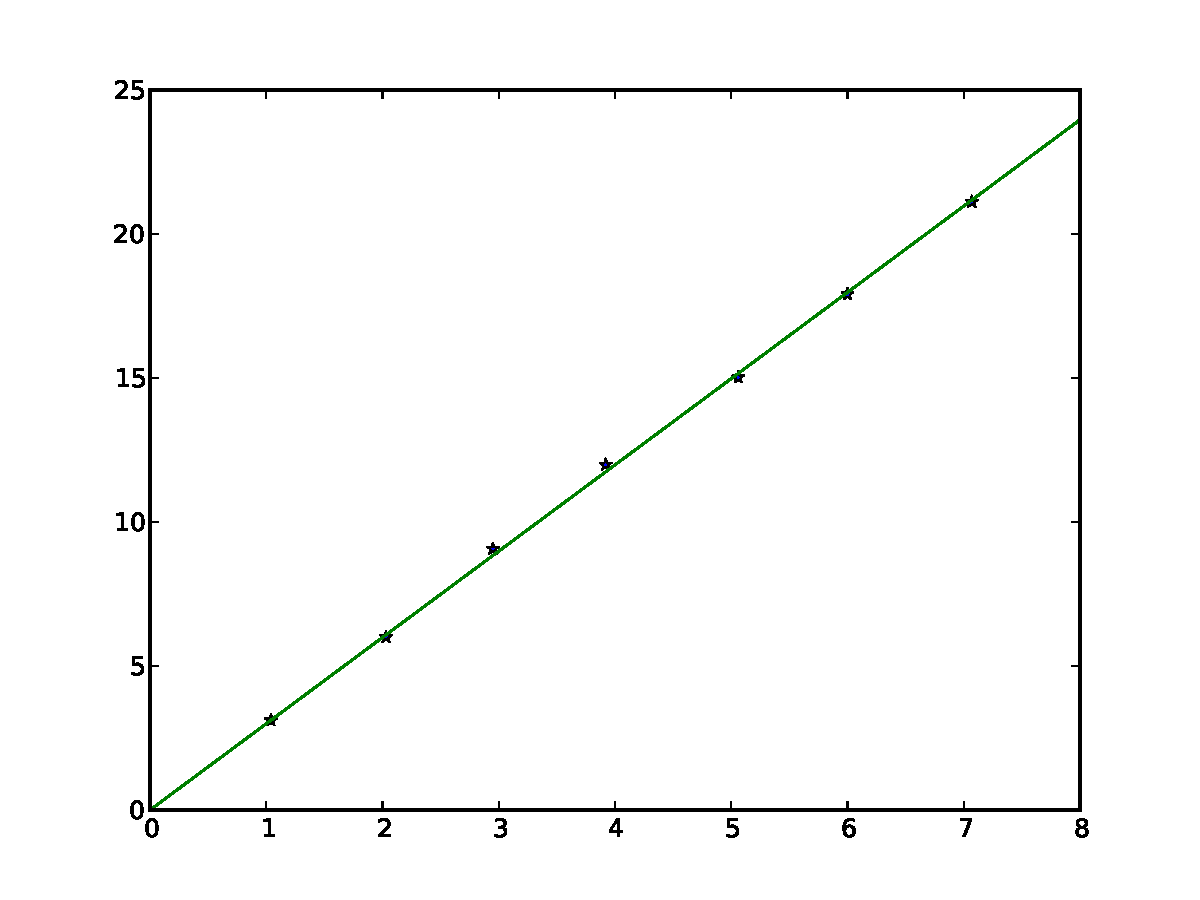
\includegraphics[scale = .6]{lab9_line_py}
\caption{The graph of the spring data together with its linear fit}
\label{Fig:SpringFit}
\end{center}
\end{figure}

\begin{lstlisting}[style=python]
: x0 = sp.linspace(0,8,100)
: y0 = k[0]*x0
: from matplotlib import pyplot as plt
: plt.plot(A,b,'*',x0,y0)
: plt.show()
\end{lstlisting}
See Figure \ref{Fig:SpringFit} to see how well the line fits the data.


\section*{General Line Fitting}

Suppose that we wish to fit a general line, that is $y=m x+b$, to the data set $\{(x_k,y_k)\}^n_{k=1}$.  Assume that the line does not cross through the origin, as in the previous example.  Then we seek both a slope and a $y$-intercept.  In this case, we set up the following linear system $A x = b$, or more precisely
\[
\begin{pmatrix}
x_1 & 1\\
x_2 & 1\\
x_3 & 1\\
\vdots & \vdots\\
x_n & 1
\end{pmatrix}
\begin{pmatrix}
m\\
b
\end{pmatrix}=
\begin{pmatrix}
y_1\\
y_2\\
y_3\\
\vdots\\
y_n
\end{pmatrix}.
\]
Note that $A$ has rank $2$ as long as not all of the $x_k$ values are the same.  Hence, the least squares solution will fit the best line for this data.


\begin{problem}
Download the file lab9.txt from the following link:
\url{http://www.math.byu.edu/~jeffh/teaching/m343h/lab9.txt}
You can load this datafile by typing
\li{lab9 = sp.genfromtxt("lab9.txt")}
Now the data is available in the array \li{lab9}.
This consists of two columns corresponding to the $x$ and $y$ values of a given data set.  Use least squares to find the slope and $y$-intercept that best fits the data.  Then plot the data points and the line on the same graph.  Finish off the problem with a discussion of what you've learned.
\end{problem}

\section*{The Cholesky Decomposition}

For certain circumstances, we have a more efficient alternative to the LU decomposition.  The Cholesky decomposition requires half the number of calculations and half the memory that the standard LU decomposition needs.  Furthermore, it is a numerically stable decomposition, which makes it all the more useful.  Because of the efficiency and numerical stability, Cholesky decomposition is used in solving least squares, optimization, and state estimation problems.  The Cholesky decomposition, however, is only applicable for positive definite matrices (symmetric matrices with strictly positive eigenvalues).  In fact, the Cholesky decomposition is an efficient way to test if a matrix is positive definite.  The Cholesky decomposition of a positive definite matrix is unique.  Think of the Cholesky decomposition as the matrix equivalent taking the square root of a positive real number.

The Cholesky decomposition of a $A$ is an lower-triangular matrix, $L$, such that
\begin{equation*}
 A = LL^H
\end{equation*}

where the entries of $L$ are calculated as follows.
\begin{align*}
&L_{i,j} = \frac{1}{L_{j,j}}\left(A_{i,j} -\sum_{k=1}^{j-1}{L_{i,k}L_{j,k}^*}\right) \mbox{ for $i>j$} \\ \\
&L_{i,i} = \sqrt{A_{i,i} - \sum_{k=1}^{i-1}{L_{i,k}L_{i,k}^*}}
\end{align*}
where $L^*$ denotes the conjugate transpose of $L$.

This is an iterative process where the current calculation may depend on previous calculations.  To calculate $L$ properly, you must start in the upper left corner and iterate down.


\begin{problem}
Write your own implementation of the Cholesky decomposition. Test it using a random symmetric matrix (build a random square matrix $A$, then $A^TA$ will be positive definite). Check the output of your function to ensure that it is functioning properly.
\end{problem}

A classical way of solving the least squares problem is to use the Cholesky decomposition, thus reducing the problem to 
\begin{equation*}
 L^HLx=A^Hb
\end{equation*}
where $L$ is the Cholesky decomposition of $A^HA$.\\
The method to do this is as follows:
\begin{enumerate}
\item[1.] Form the matrix $A^HA$ and the vector $A^Hb$.
\item[2.] Compute the Cholesky factorization $A^HA=L^HL$.
\item[3.] Solve the lower-triangular system $L^Hw=A^Hb$ for $w$.
\item[4.] Solve the upper-triangular system $Lx=w$ for $x$.
\end{enumerate}



\begin{comment}
algorithm taken from Trefethen, Numerical Linear Algebra pg. 82
\end{comment}


\begin{problem}
Use your implementation of Cholesky decomposition to solve problem 2.
\end{problem}



\begin{comment}
\begin{problem}
Compare how your Cholesky decomposition performs against your LU decomposition from Lab \ref{lab:LUdecomp}.  Perform the following comparisons by decomposing increasingly large positive definite matrices.  Plot the comparison results.
\begin{itemize}
 \item Runtime: Time how long each decomposition needs to decompose the input matrix.
 \item Operations: Count the number of operations needed to compute each decomposition.  This can be done by adding a line in the loop to count each time an operation occurs.
\end{itemize}
\end{problem}
\end{comment}